\documentclass{article}

\usepackage{amsmath}
\usepackage{graphicx}

\title{Phase coexistence in the van der Waals system}

\author{Sebastian G. Winther-Larsen}

\date{\today}

\begin{document}

\maketitle

\section*{a)}
The ideal gas equation is 
\begin{equation}
\label{eq:idealgas}
PV = nRT
\end{equation}
where $P$ is the pressure, $V$ is the volume, $n$ is the number of molecules, $R=kN_a$ is a product of Boltzmann's constant and the Avogadro's constant and $T$ is the temperature of the gas. The \emph{van der Waals} equation makes two modifications tot he ideal gas law in equation \ref{eq:idealgas}, adding $aN^2/V^2$ to $P$ and subtracting $Nb$ from $V$. The first modification accounts for short range attraction between molecules when they're not touching and the second modification is supplies the condition that the volume of the gas is greater than zero. Employing the relation $nR=Nk$ and the before-mentioned modifications gives us the van der Waals equation
\begin{equation}
\label{eq:vanderwaals}
\left(p + \frac{aN^2}{V^2}\right)(V-Nb) = NkT
\end{equation}

The potential energy is associated with each particles interaction with its neighbour is proportional to the density of particles $N/V$. The total potential energy associated with all molecules' interaction must then be proportional to $N^2/V$, since there are $N$ molecules.
\begin{equation}
U_{tot} = -\frac{aN^2}{V}
\end{equation}
where $a$ is simply some constant which depends on the types of molecules in the gas. Now, if one would vary the volume $V$ slightly, while hoping the entropy $S$ remains fixed, the relation $dU = -PdV$ holds, giving
\begin{equation}
\label{eg:Upressure}
p_{U} = -\left(\frac{dU}{dV}\right)_S = -\frac{d}{dv}\left(-\frac{aN^2}{V} \right) = -\frac{aN^2}{V^2}
\end{equation}
In absence of attractive forces, the pressure of the fluid would be $NkT/(V-Nb)$, rewriting the ideal gas law and using the effective volume. Adding this to the pressure from equation \ref{eg:Upressure} we land at  
\begin{equation}
\label{eq:vdwpressure}
p = \frac{NkT}{V-Nb}-\frac{aN^2}{V^2}
\end{equation}
which is equation \ref{eq:vanderwaals} rewritten in terms of pressure, called the equation of state for a van der Waals gas.

\section*{b)}
Now, we want to make equation \ref{eq:vdwpressure} dimensionless. This can be done by introducing the following quantities
\begin{align*}
\hat{p} = \frac{p}{p_c}, \quad &\hat{V} = \frac{V}{V_c}, \quad \hat{T} = \frac{T}{T_c}, \\
p_c = \frac{a}{27b^2}, \quad &V_c = 3Nb, \quad kT_c = \frac{8a}{27b}
\end{align*}
Applying them where needed
\begin{align*}
\hat{p} = \frac{27b^2NkT}{a(V-Nb)} &- \frac{27b^2aN^2}{aV^2} \\
		= \frac{27b^2NkT_c\hat{T}}{a(\hat{V}V_c-\frac{1}{3}V_c)} &- \frac{27b^2N^2}{\hat{V}^2V_c^2} \\
		= \frac{8bN\hat{T}}{\hat{V}V_c-\frac{1}{3}V_c} &- \frac{3V_c^2}{\hat{V}^2V_c^2} \\
		= \frac{8\hat{T}}{3\hat{V}^2-1} &- \frac{3}{\hat{V}^2}.
\end{align*}
We have landed at a neat dimensionless expression.

\section*{c)}
\begin{figure}
	\centering
	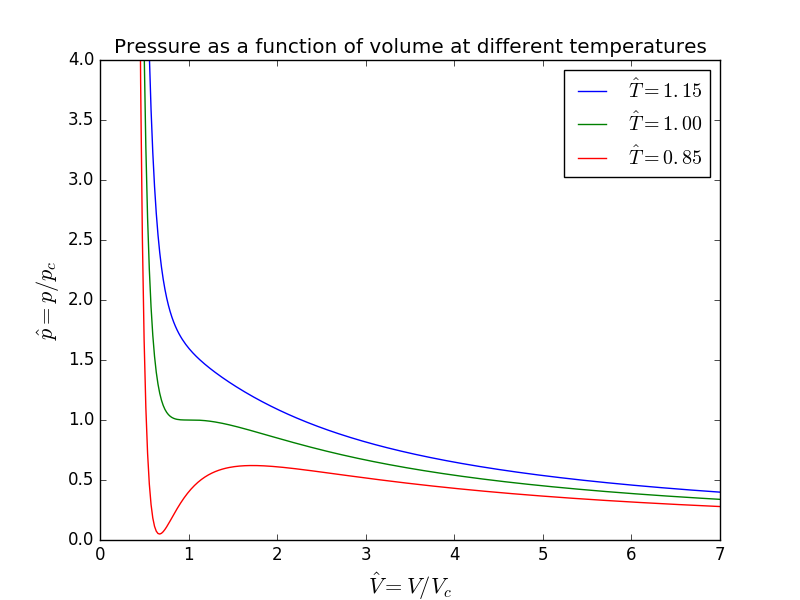
\includegraphics[width=0.9\textwidth]{figures/pressureVsVolume.png}
	\caption{The dimensionless pressure $\hat{p}$ of the system as a function of the dimensionless volume $\hat{V}$ for different temperatures $\hat{T}$.}
	\label{fig:pressureVsVolume}
\end{figure}

Figure \ref{fig:pressureVsVolume} show the dimensionless pressure $\hat{p}$ as a function of dimensionless volume $\hat{V}$. One can see that for temperatures $\hat{T} < 1$ the pressure value is not uniquely mapped to a single value for volume. It would therefore be impossible to find $\hat{V}(\hat{p})$.

\section*{d)}
The dimensionless pressure can also be written in terms of dimensionless density $\hat{\rho}$ using the following quantities
\begin{align*}
\hat{\rho}=\frac{1}{\hat{V}}=\frac{\rho}{\rho_c}, \quad \rho_c = \frac{1}{3b}.
\end{align*}
Inserting these into equation \ref{eq:vdwpressure} where needed
\begin{align}
\hat{p} = \frac{27b^2NkT}{a(V-Nb)} &- \frac{27b^2N^2}{V^2} \nonumber\\
		= \frac{8Nb\hat{T}}{V-Nb} &-\frac{3V_c^2}{V_c^2}\hat{\rho}^2 \nonumber\\
		= \frac{V8\hat{\rho}\hat{T}}{V(3-\hat{\rho})} &- 3\hat{\rho}^2 \nonumber\\
		= \frac{8\rho\hat{T}}{3-\hat{\rho}} &- 3\hat{\rho}^2 \label{eq:dimlessdensity}
\end{align}
Again a neat dimensionless expression.

\section*{e, f)}
\begin{figure}
	\centering
	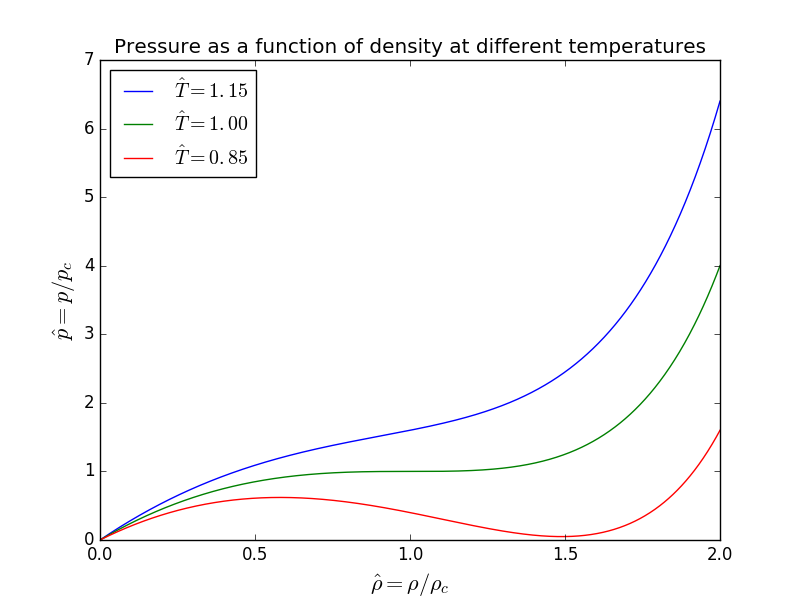
\includegraphics[width=0.9\textwidth]{figures/pressureVsDensity.png}
	\caption{The dimensionless pressure $\hat{p}$ of the system as a function of the dimensionless density $\hat{\rho}$ for different temperatures $\hat{T}$.}
	\label{fig:pressureVsDensity}
\end{figure}

Figure \ref{fig:pressureVsDensity} shows the dimensionless pressure $\hat{p}$ plotted against dimensionless density $\hat{\rho}$. One can easily see that $\hat{T}>1$ gives a unique function for pressure, i.e. $T>T_c$, as was the case for the pressure as a function of volume in the previous two problems.

\section*{g)}
Isothermic compressibility is defined as
\begin{equation}
\label{eq:isoComp}
\kappa = -\frac{1}{V}\left(\frac{\partial V}{\partial p} \right)_{T,N} = \frac{1}{\rho}\left(\frac{\partial \rho}{\partial p} \right)_{T,N}
\end{equation}
One can see from figure \ref{fig:pressureVsVolume} that the isothermic compressibility becomes negative whenever the pressure versus volume curve slopes upwards. This can only happen when $\hat{T} < 1$. In figure \ref{fig:pressureVsDensity} the isothermic compressibility is negative when the pressure versus density curve slopes downwards. Here this can also only happen when $\hat{T} < 1$. A negative compressibility means that the system is unstable.

\section*{h)}
Helmholtz free energy for a van der Waals gas i given by
\begin{equation}
F_{vdW} = -NkT\left(\ln \left( \frac{n_Q(V-Nb)}{N} \right) + 1 \right) - \frac{aN^2}{V},
\end{equation}
where $n_Q(T) = (2\pi mkT/h^2)^{3/2}$. In general Helmholtz free energy is $F = U - TS$, while Gibbs free energy is $G = U + pV - TS$ alternatively $G = F + pV$ where, in this particular case
\begin{equation}
\label{eq:pV}
pV = \frac{NkTV}{V-Nb}-\frac{aN^2}{V},
\end{equation}
and one can easily see that Gibbs free energy for a van der Waals gas must be
\begin{equation}
\label{eq:GvdW1}
G_{vdW} = \frac{NkTV}{V-Nb} -\frac{2aN^2}{V} - NkT\left(\ln \left( \frac{n_Q(V-Nb)}{N} \right) + 1 \right)
\end{equation}

\section*{i)}
One can find an alternative expression for Gibbs free energy by way of the thermodynamic identity for $G$
\begin{equation}
dG = -SdT + VdP - \mu dN
\end{equation}
For a fixed temperature and a given number of molecules this equation reduces to $dG = VdP$, dividing both sides by $dV$ gives
\begin{align*}
\left(\frac{\partial G}{\partial V}\right)_{N,T} &= V \left(\frac{\partial P}{\partial V} \right)_{N,T} \\
\left(\frac{\partial G}{\partial V}\right)_{N,T} &= V \left(-\frac{NkT}{(V-Nb)^2} + \frac{2N^2}{V^3} \right) \\
\left(\frac{\partial G}{\partial V}\right)_{N,T} &= -\frac{NkTV}{(V-Nb)^2} + \frac{2N^2}{V^2} \\
G &= -NkT \ln (V-Nb) - \frac{NkT}{V-Nb} - \frac{2aN^2}{V} + c'(T)
\end{align*}
Once can rewrite the constant such that $c'(T) = NkTc(T)$ and insert for $pV$ (equation \ref{eq:pV}) in order to get
\begin{equation}
\label{eq:GvdW2}
G = -NkT\ln (V-Nb) - \frac{aN^2}{V} + pV + NkTc(T)
\end{equation}
One will arrive at this expression by rewriting equation \ref{eq:GvdW1} directly as well.

\section*{j)}
It can be beneficial to rewrite Gibbs free energy to a dimensionless expression. To do this one will need $G_c = 3kT_c/8$. Gibbs free energy per molecule is $\hat{g} = (G/G_c)/N$. I will equate one part of equation \ref{eq:GvdW2} at at time.
\begin{align*}
& -NkT\ln (V-Nb) \frac{1}{G_cN} = -\frac{8NkT}{3kT_cN}\ln (V-Nb) = -\frac{8}{3} \hat{T}\ln(V-Nb) \\
& -\frac{8}{3}\hat{T} \ln (\hat{V}V_c - \frac{1}{3}V_c) = -\frac{8}{3}\hat{T} \ln (3\hat{V}-1) - \frac{8}{3}\hat{T}\ln(\frac{V_c}{3})
\end{align*}
Singe I'm only interested in terms that depend on $\hat{p}$ and $\hat{\rho}$ I will ignore the second term. So the first term in equation \ref{eq:GvdW2} becomes
\begin{equation}
\label{eq:term1}
-\frac{8}{3}\hat{T}\ln \left(\frac{3}{\hat{\rho}}-1 \right)
\end{equation}
The constant only depends on $T$ and can also be ignored. The last two parts are
\begin{align*}
&\left(pV - \frac{aN^2}{V} \right) \frac{1}{G_c N}= \left(\frac{NkTV}{V-Nb} - \frac{2aN}{V} \right) \frac{1}{G_c N} \\
&= \frac{8\hat{T}V}{3V-VNb} - \frac{16}{3}\frac{2aN}{kT_cV} = \frac{8\hat{T}V}{3V-\hat{\rho}V} -\frac{16}{3}\frac{27b}{8a}\frac{aN}{V} \\
&=\frac{8\hat{T}}{3-\hat{\rho}} - (2)(9)\frac{bN}{V}
\end{align*}
The first part is done, but the second still needs some work.
\begin{equation*}
- (2)(9)\frac{bN}{V} = - (2)(9)\frac{bN}{\hat{V}V_c} = - (2)(9)\frac{bN}{\hat{V}3Nb}= - (2)(3)\frac{1}{V} = -(2)(3) \hat{\rho}
\end{equation*}
then these last two terms become 
\begin{equation*}
\frac{8\hat{T}}{3-\hat{\rho}} - 3\hat{\rho} - 3\hat{\rho}
\end{equation*}
which one can write, using equation \ref{eq:dimlessdensity}, as
\begin{equation}
\label{eq:term2}
\frac{\hat{p}}{\hat{\rho}} - 3\hat{\rho}
\end{equation}
combining equations \ref{eq:term1} and \ref{eq:term2} yields the dimensionless form of Gibbs free energy per molecule
\begin{equation}
\hat{g} = \frac{G/G_c}{N} = -3\hat{\rho} -\frac{8}{3}\hat{T}\ln \left( \frac{3}{\hat{\rho}} - 1 \right) + \frac{\hat{p}}{\hat{\rho}}
\end{equation}

\section*{k)}

\end{document}